\documentclass[border=2pt]{standalone}
\usepackage{pgfplots}
\pgfplotsset{compat=1.18}
\begin{document}
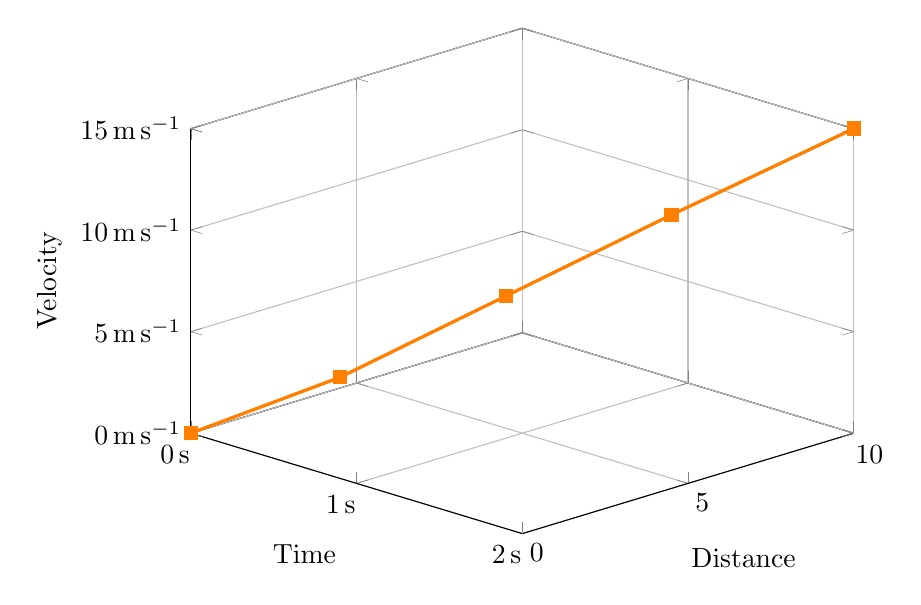
\begin{tikzpicture}
  \begin{axis}[
    width=10cm,
    height=8cm,
    view={45}{25},
    xmin=0,
    xmax=2,
    ymin=0,
    ymax=2,
    zmin=0,
    zmax=15,
    xtick={0,1,2},
    xticklabel={$\pgfmathprintnumber{\tick}\,\mathrm{s}$},
    ytick={0,1,2},
    yticklabels={$0$,$5$,$10$},
    ztick={0,5,10,15},
    zticklabel={$\pgfmathprintnumber{\tick}\,\mathrm{m\,s^{-1}}$},
    grid=major,
    xlabel={Time},
    ylabel={Distance},
    zlabel={Velocity}
  ]
    \addplot3[orange,very thick,mark=square*] coordinates {
      (0,0,0) (0.5,0.4,3) (1,0.9,7) (1.5,1.4,11) (2,2,15)
    };
  \end{axis}
\end{tikzpicture}
\end{document}
